\setchapterpreamble[u]{\margintoc}

\chapter{Introduction}
\labch{intro}

\begin{fullwidth}
\begin{quote}
  {\itshape ``Solving a mystery is not the same as deducing from first principles. Nor
does it amount simply to collecting a number of particular data from which to infer a general law. It
means, rather, facing one or two or three particular data apparently with nothing in common, and
trying to imagine whether they could represent so many instances of a general law you don’t yet
know, and which perhaps has never been pronounced.``}
  \begin{flushright}
    Umberto Eco, {\sffamily\color{ming} The Name of the Rose}
  \end{flushright}
\end{quote}
\end{fullwidth}

\vspace{1cm}

Relativistic heavy-ion collisions provide the means to study a multitude of phenomena.\sidenote{Such as collective flow \cite{Shuryak:2004cy}, jet quenching \cite{Wang:1991xy} and many others.}From a theoretical point of view, these collisions may be described within effective theories. Nevertheless, trying to grasp a unitary physical picture from a mosaic of disjoint theories is extremely difficult. 

\begin{figure*}[!hbt]
	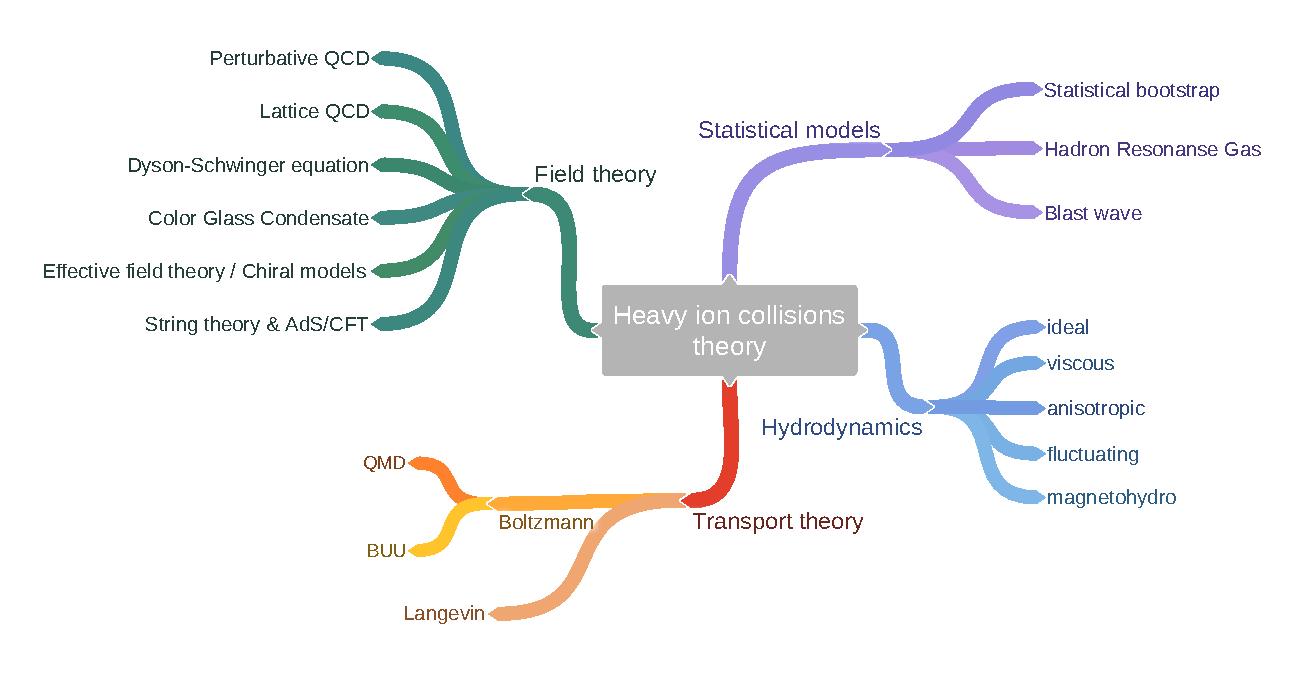
\includegraphics[width=1.5\textwidth]{images/Heavy_ion_collisionstheory.pdf}
	\caption{\normalsize Various theoretical models which aim to describe different aspect of heavy-ion collisions. Diagram taken from \cite{Oliinychenko:2017sfl}.} 
\end{figure*}

The ultimate test is the comparison to experimentally measured data, which may not be done using a single effective theory. For this reason, {\sffamily\color{ming} hybrid} approaches\sidenote{See for example \cite{Bernhard:2016tnd, ryuimpbulk, Devetak:2019lsk}.}are more suitable. They consists in coupling various theoretical descriptions, each within its appropriate range of applicability, and reconstruct heavy-ion collisions stage by stage.

\begin{figure}[!hbt]
	\centering
    \includesvg[width=0.9\textwidth]{images/diagrams/stages.svg}
    \caption{\normalsize Light-cone diagram revealing different stages of heavy-ion collisions. The idea for such a representation is borrowed from \cite{Gelis:2012ri}.}
\end{figure}

\fancybox{customgray}{{\color{customgray}\sffamily Before collision}\\ $\tau<\tau_\text{col}$}{
Before the collision, the nuclei propagate along the light-cone. They may be described using the {\sffamily CGC} model, constructed as a high-energy limit of {\sffamily QCD}.
}

\fancybox{tealblue}{{\color{tealblue}\sffamily Initial stage}\\ $\tau_\text{col}<\tau<\tau_\text{sat}$}{
Immediately after the collision, a state of matter referred to as the Glasma, which consists of strong classical color fields, is produced in the forward light-cone.
}

\fancybox{crem}{{\color{crem}\sffamily Thermalization}\\ $\tau_\text{sat}<\tau<\tau_\text{eq}$}{
The pre-equilibrium matter resulting from the initial stage undergoes a process of fast thermalization, described within an effective kinetic theory approach.
}

\fancybox{lightgreen}{{\color{lightgreen}\sffamily QGP transport}\\ $\tau_\text{eq}<\tau<\tau_\text{fo}$}{
The {\sffamily QGP} expands due to pressure gradients. This evolution may successfully be modeled with ideal or viscous relativistic hydrodynamics. 
}

\fancybox{ming}{{\color{ming}\sffamily Hadronization}\\ $\tau_\text{fo}<\tau<\tau_\text{dec}$}{
Once the critical {\sffamily QCD} phase transition temperature is reached, the deconfined quarks and gluons recombine intro hadrons.
}

\fancybox{darkblue}{{\color{darkblue}\sffamily Free streaming}\\ $\tau<\tau_\text{det}$}{
When all interactions among hadrons cease, kinetic freeze-out is reached. After the decoupling takes place, produced particles free stream towards the detectors.
}

In this thesis, a modest hybrid simulation approach is presented: initial conditions obtained from the {\sffamily MV} model and implemented using real-time lattice gauge theory\sidenote{Simulated with {\sffamily Curraun}.}are coupled to relativistic viscous hydrodynamics\sidenote{Implemented in {\sffamily MUSIC}.} and afterwards compared to experimental data\sidenote{For {\sffamily Au-Au} collision with $\sqrt{s_\textsf{NN}}=200$ GeV from {\sffamily RHIC}.}.